\documentclass[oneside, 11pt]{article}

\usepackage[T1]{fontenc}
\usepackage[utf8]{inputenc}
\usepackage[dutch]{babel}

\usepackage{fouriernc}
\usepackage[detect-all, load-configurations=binary,
            separate-uncertainty=true, per-mode=symbol,
            retain-explicit-plus, range-phrase={ tot }]{siunitx}

\usepackage{setspace}
\setstretch{1.2}

\setlength{\parskip}{\smallskipamount}
\setlength{\parindent}{0pt}

\usepackage{geometry}
\geometry{marginparwidth=0.5cm, verbose, a4paper, tmargin=3cm, bmargin=3cm, lmargin=2cm, rmargin=2cm}

\usepackage{float}

\usepackage[fleqn]{amsmath}
\numberwithin{equation}{section}
\numberwithin{figure}{section}

\usepackage{graphicx}
\graphicspath{{Figures/}}
\usepackage{subfig}

\usepackage{tikz}
\usetikzlibrary{plotmarks}

\usepackage{fancyhdr}
\pagestyle{fancy}
\fancyhf{}
\rhead{\thepage}
\renewcommand{\footrulewidth}{0pt}
\renewcommand{\headrulewidth}{0pt}

\usepackage{relsize}
\usepackage{xspace}
\usepackage{url}

\newcommand{\figref}[1]{Figuur~\ref{#1}}

\newcommand{\hisparc}{\textsmaller{HiSPARC}\xspace}
\newcommand{\kascade}{\textsmaller{KASCADE}\xspace}
\newcommand{\sapphire}{\textsmaller{SAPPHiRE}\xspace}
\newcommand{\jsparc}{\textsmaller{jSparc}\xspace}
\newcommand{\hdf}{\textsmaller{HDF5}\xspace}
\newcommand{\aires}{\textsmaller{AIRES}\xspace}
\newcommand{\csv}{\textsmaller{CSV}\xspace}
\newcommand{\python}{\textsmaller{PYTHON}\xspace}
\newcommand{\corsika}{\textsmaller{CORSIKA}\xspace}
\newcommand{\labview}{\textsmaller{LabVIEW}\xspace}
\newcommand{\daq}{\textsmaller{DAQ}\xspace}
\newcommand{\adc}{\textsmaller{ADC}\xspace}
\newcommand{\adcs}{\textsmaller{ADC}s\xspace}
\newcommand{\Adcs}{A\textsmaller{DC}s\xspace}
\newcommand{\hi}{\textsc{h i}\xspace}
\newcommand{\hii}{\textsc{h ii}\xspace}
\newcommand{\mip}{\textsmaller{MIP}\xspace}
\newcommand{\hisparcii}{\textsmaller{HiSPARC II}\xspace}
\newcommand{\hisparciii}{\textsmaller{HiSPARC III}\xspace}
\newcommand{\pmt}{\textsmaller{PMT}\xspace}
\newcommand{\pmts}{\textsmaller{PMT}s\xspace}

\DeclareSIUnit{\electronvolt}{\ensuremath{\mathrm{e\!\!\:V}}}

\DeclareSIUnit{\unitsigma}{\ensuremath{\sigma}}
\DeclareSIUnit{\mip}{\textsmaller{MIP}}
\DeclareSIUnit{\adc}{\textsmaller{ADC}}

\DeclareSIUnit{\gauss}{G}
\DeclareSIUnit{\parsec}{pc}
\DeclareSIUnit{\year}{yr}


\usepackage{xfrac}

\title{Stationsonderhoud}
\author{C.G.N. van Veen}
\docrecept{1}{SO}
\version{1.0}

\begin{document}

\maketitle

\section{Inleiding}

Deze lesbrief gaat in op het onderhoud van een \hisparc station.
Leerlingen krijgen eerst een introductie over kosmische straling en gaan
dan aan de slag met het analyseren van een \hisparc station en
uiteindelijk stellen de leerlingen het station optimaal in. Er is
achtergrond materiaal beschikbaar op
\url{http://www.hisparc.nl/docent-student/lesmateriaal/informatie-pakket/} en
op \url{http://www.hisparc.nl/docent-student/lesmateriaal/routenetpad/} respectievelijk
het \textit{infopakket} en \textit{routenet}.

De lessenserie van 3 lessen is als volgt opgebouwd:
\begin{description}
    \item[Les 1] Introductie over kosmische straling, bijhorende terminologie en metingen van \hisparc.
    Bij les 1 hoort een werkblad.

    \item[Les 2] Les over hoe de stations meten, hoe deze meten en wat er af te lezen valt van
    histogrammen op: \url{http://data.hisparc.nl}.
    Bij les 2 hoort een werkblad.

    \item[Les 3] Onderhoud en instellen station
    In deze les leren de leerlingen iets over de instelling van het \hisparc station.
    Zij gaan de fotomultipliers van de detectoren instellen en de resultaten van
    hun instellingen bekijken. Bij les 3 hoort een opgaveblad.
\end{description}

Opmerking: leerlingen hebben bij deze lessenserie baat bij kennis van
elektrische velden, versnelspanning, energie van fotonen, radioactief verval,
deeltjesfysica en de lorentzfactor ($\gamma$):
\begin{equation}
    E = h \cdot f
\end{equation}
\begin{equation}
    q \cdot {U_{AK}} = \sfrac{1}{2} \cdot m \cdot {v^2}
\end{equation}
\begin{equation}
    \gamma = \frac{1}{\sqrt{1-\frac{v^2}{c^2}}}
\end{equation}

\section{Les 1}

Als docent kunt u een aantal invalshoeken kiezen om de introductie van
kosmische straling aan te bieden.  In deze les starten we met
achtergrond materiaal en een werkblad. Tijdens deze les kunnen
leerlingen ook een station bezoeken als dat op school staat. Belangrijk
is dat er een introductie op kosmische straling gegeven wordt en dat de
terminologie duidelijk wordt gemaakt.
Behandel in ieder geval:
\begin{itemize}
    \item Wat is kosmische straling?
    \item Hoe ontstaat een deeltjeslawine? 
    \item Hoe worden deze deeltjes in de lawine op aarde gedetecteerd?
\end{itemize}

\textbf{Achtergrondmateriaal}
Uit het infopakket, onder de kop
Algemeen:\textit{Terminologie, Cosmic air showers} en$/$of \textit{ Uitleg \hisparc}.

\textbf{Werkblad} Het werkblad `Cosmic air showers' kan uitgedeeld worden aan
leerlingen. Deze is te vinden in het infopakket.
\textit{Werkblad-2}. Kies het werkblad `kosmische straling'.
De opgaven van dit stencil kunnen door de leerlingen zelfstandig gemaakt worden.

\textbf{Opmerking:}
Van de \hisparc site (\url{www.hisparc.nl}) kunnen diverse bestaande powerpoint-presentaties
gedownload worden.
Deze presentaties mogen naar believen aangepast worden, om door leerlingen en docenten
in de klas te gebruiken.

\section{Les 2}
In deze les gaan we naar de meetstations van \hisparc kijken en met name naar de
afstelling van de detectoren en het onderhoud van een station.
We beginnen met achtergrondinformatie over de detectoren. In deze les is het 
belangrijk dat in ieder geval pulshoogte-histogram uitgelegd wordt en hoe dit histogram
gemaakt wordt.

In deze les behandelen we zaken als:
\begin{itemize}
    \item Hoe meten de detectoren de deeltjes in de lawine?
    \item Wat is het pulshoogte-histogram?
    \item Hoe kunnen we foutmeldingen opsporen en oplossingen vinden?
\end{itemize}

\textbf{Achtergrondmateriaal}
Uit het infopakket: \textit{Inregelen
PMT's}, \textit{Controle station} en \textit{Uitleg \hisparc}. 
In het document `controle station' wordt uitgelegd hoe leerlingen zelf
problemen met stations kunnen constateren en oplossen. Vooral een
pulshoogte diagram, die er uitziet als in figuur 3.1 in dit document is
een probleem wat leerlingen zelf kunnen oplossen.

\textbf{Werkblad}
Kies van Routenet:
\textit{Detecteren} en \textit{Detector}:
De opgaven van deze bladen kunnen in de les gemaakt worden.

\section{Les 3}
In deze les kijken we naar de DAQ software van het meetstation en gaan de leerlingen
zelf aan de slag met het instellen van de fotomultipliers (PMT's) van het station.
De leerlingen krijgen wat (meer) uitleg over de fotomultiplier en stellen via de \hisparc \daq
de juiste spanning in voor fotomultiplier.

In deze les behandelen we zaken als:
\begin{itemize}
    \item Hoe werkt een fotomultiplierbuis? 
    \item Hoe kunnen we de spanning op de stations zo instellen dat er een
    goed pulshoogte diagram ontstaat?
\end{itemize}

\textbf{Achtergrondmateriaal}
In infopakket staat het document \textit{inregelen PMTs},
waarin een uitleg wordt gegeven van de werking van de fotomultiplier buis.

In het document \textit{inregelen PMTs} wordt naast de werking van de fotomultiplier
ook de instelling van de \hisparc \daq uitgelegd. Leerlingen kunnen dit gebruiken om
de instellingen van de PMT's van de detectors van het \hisparc station.

\textbf{Korte handleiding} Hieronder staat een lijst van de handelingen. 
Het verdient sterke aanbeveling om het hele document `inregelen PMT's' te lezen!

\begin{itemize}
    \item Zorg dat de \daq mode stopt. (dit betekent dat er geen data meer wordt verzonden.)
    \item Zorg dat je de adc alignment het gedaan, voor \hisparc III \daq wordt de common offset
    10
    \item Stel de spanning van de PMT in (vanaf 300 V beginnen!) Zie \figref{fig:PMT_instellen}.
    \item Test de spanning in het menu "statistics (trace\&trigger)", klik `start counting'.)
    \item De PMT is goed ingesteld op het moment, dat de `average per second (HIGH)' 
    op ongeveer 120 komt en (LOW) rond de 250 uitkomt. Zie \figref{fig:instellen_PMT_values}.
    \item Pas de PMT spanning in kleine stapjes aan om deze waarden te verkrijgen. Klik na elke aanpassing op `save settings'
    \item Herhaal de meting tot dat de instellingen de juiste `average per second' hebben bereikt.
    \item De PMT is nu juist ingesteld.
\end{itemize}

\begin{figure}
    \centering
    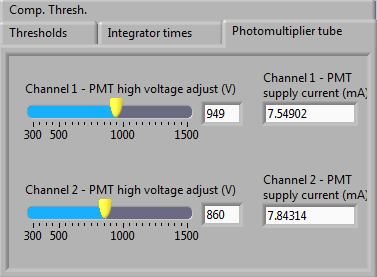
\includegraphics[scale=0.4]{PMT_instellen}
    \caption{In dit tab menu kan de spanning op de fotobuis worden ingesteld.
    Je kunt de slider verslepen of een spanning invoeren in het vakje.}
    \label{fig:PMT_instellen}
\end{figure}

\begin{figure}
    \centering
    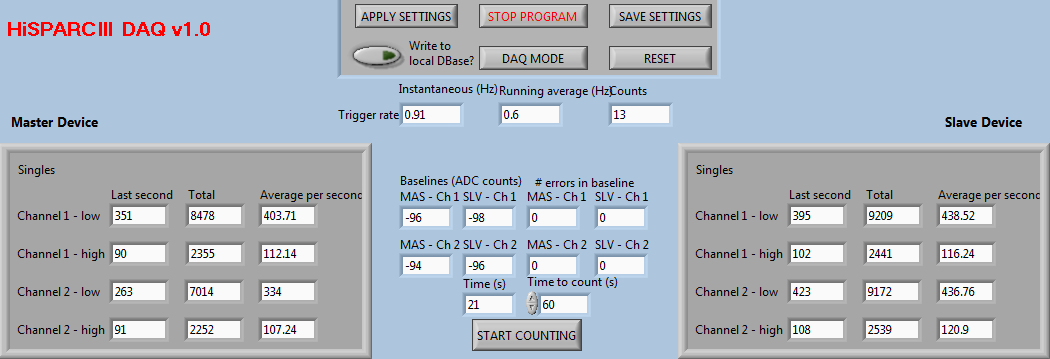
\includegraphics[scale=0.4]{instellen_PMT_values}
    \caption{In dit tab menu kun je op start counting drukken. De detectoren gaan dan meten.
    De waarden zouden voor de 3e kolom `average per second' bij `High' 120 moeten zijn en bij `low' ongeveer 250.
    Dit figuur heeft dus alleen voor detector 4 nu een goede waarde van 120.
    Daarom moet je de count ook de volledige 60 s laten lopen.}
    \label{fig:instellen_PMT_values}

\end{figure}

\textbf{Werkblad}
Leerlingen kunnen als opdracht een opgave over een fotomultiplier maken.







\end{document}
